\chapter{Propuesta}
%TODO CONTEXTO DE LO QUE VA ESTO
Para comprobar la validez de las heurísticas, se realiza un desarrollo de un audiojuego con dos modalidades. Se analizan sus requisitos, se estiman temporalmente la duración de las tareas del trabajo y se diseña y programa un juego accesible. Posteriormente, se realizan pruebas de usuario que se analizan a través de las heurísticas en el capítulo de conclusiones.
\section{Especificación de requisitos}
% TODO redactar metodología
Seguidamente se van a listar los requisitos funcionales (RF), no funcionales
(RNF) y requisitos de información (RI) de este juego, que comprenden las acciones que los jugadores tomarán para interactuar con la aplicación.
\subsection{Requisitos funcionales}
Los requisitos funcionales describen las acciones que el juego debe realizar para asegurar una correcta ejecución. 

\begin{table}[H]
	\centering
	\caption{RF-1 - Iniciar juego.}
	\label{table:RF1}
	\begin{tabular}{|l|p{10cm}|}
		\hline
		\multicolumn{2}{|c|}{\textbf{RF-1 - Iniciar juego}} \\
		\hline
		\textbf{Descripción} & Abrir el juego y mostrar interfaz inicial. \\
		\hline
		\textbf{Prioridad} & Alta \\
		\hline
		\textbf{Datos de entrada} & Ninguno \\
		\hline
		\textbf{Prerrequisitos} & Juego instalado en el sistema que vaya a ejecutarlo. \\
		\hline
		\textbf{Procesamiento} & Se inicia el juego y se muestra el menú principal. \\
		\hline
		\textbf{Postcondición} & Al usuario se le presenta un menú con las opciones de iniciar el juego, acceder al menú de opciones y salir. \\
		\hline
	\end{tabular}
	
\end{table}
\begin{table}[H]
	\centering
	\caption{RF-2 - Finalizar juego.}
	\label{table:RF2}
	\begin{tabular}{|l|p{10cm}|}
		\hline
		\multicolumn{2}{|c|}{\textbf{RF-2 - Finalizar juego}} \\
		\hline
		\textbf{Descripción} & Cerrar la aplicación y sus interfaces. \\
		\hline
		\textbf{Prioridad} & Alta \\
		\hline
		\textbf{Datos de entrada} & Ninguno \\
		\hline
		\textbf{Prerrequisitos} & Usuario en el menú principal del juego. \\
		\hline
		\textbf{Procesamiento} & Se pide al usuario una confirmación de salida. Tras confirmar, se cierra el juego. \\
		\hline
		\textbf{Postcondición} & El usuario confirma la salida del juego y cierra la aplicación. \\
		\hline
	\end{tabular}
	
\end{table}
\begin{table}[H]
	\centering
	\caption{RF-3 - Cambiar configuración de audio.}
	\label{table:RF3}
	\begin{tabular}{|l|p{10cm}|}
		\hline
		\multicolumn{2}{|c|}{\textbf{RF-3 - Cambiar configuración de audio}} \\
		\hline
		\textbf{Descripción} & Permitir modificar los niveles de volumen de los distintos tipos de audio de la aplicación desde el menú de configuración.  \\
		\hline
		\textbf{Prioridad} & Media \\
		\hline
		\textbf{Datos de entrada} & Valor de configuración de volumen aportado por usuario. \\
		\hline
		\textbf{Prerrequisitos} & Usuario en menú de configuración. \\
		\hline
		\textbf{Procesamiento} & Se almacena el volumen en preferencias de usuario y se modifican los decibelios de los buses de audio del juego. \\
		\hline
		\textbf{Postcondición} & El usuario recibirá un sonido de confirmación en el volumen seleccionado. \\
		\hline
	\end{tabular}
	
\end{table}
\begin{table}[H]
	\centering
	\caption{RF-4 - Visualizar configuración.}
	\label{table:RF4}
	\begin{tabular}{|l|p{10cm}|}
		\hline
		\multicolumn{2}{|c|}{\textbf{RF-4 - Visualizar configuración}} \\
		\hline
		\textbf{Descripción} & Mostrar la configuración del volumen de audio.  \\
		\hline
		\textbf{Prioridad} & Media \\
		\hline
		\textbf{Datos de entrada} & Ninguno \\
		\hline
		\textbf{Prerrequisitos} & Usuario entra en menú de configuración \\
		\hline
		\textbf{Procesamiento} & El sistema carga las preferencias de usuario en los indicadores gráficos del menú. \\
		\hline
		\textbf{Postcondición} & El usuario es capaz de ver el volumen de audio precargado y es capaz de saber el nivel interactuando con los indicadores.  \\
		\hline
	\end{tabular}
	
\end{table}
	\begin{table}[H]
		\centering
		\caption{RF-5 - Informar sobre controles.}
		\label{table:RF5}
		\begin{tabular}{|l|p{10cm}|}
			\hline
			\multicolumn{2}{|c|}{\textbf{RF-5 - Informar sobre controles}} \\
			\hline
			\textbf{Descripción} &  Indicar información sobre los controles disponibles para utilizar la aplicación.  \\
			\hline
			\textbf{Prioridad} & Baja \\
			\hline
			\textbf{Datos de entrada} & Ninguno \\
			\hline
			\textbf{Prerrequisitos} & Se ha iniciado el juego. \\
			\hline
			\textbf{Procesamiento} & Se muestra una pantalla con un temporizador indicando la información de los controles y se reproduce un audio describiéndolos. \\
			\hline
			\textbf{Postcondición} & El usuario escucha información sobre los controles con los que puede utilizar el juego. \\
			\hline
		\end{tabular}
		
	\end{table}
\begin{table}[H]
	\centering
	\caption{RF-6 - Controles intercambiables.}
	\label{table:RF6}
	\begin{tabular}{|l|p{10cm}|}
		\hline
		\multicolumn{2}{|c|}{\textbf{RF-6 - Controles intercambiables}} \\
		\hline
		\textbf{Descripción} & Permitir el cambio de mando a teclado y viceversa durante la ejecución del juego.  \\
		\hline
		\textbf{Prioridad} & Media \\
		\hline
		\textbf{Datos de entrada} & Ninguno \\
		\hline
		\textbf{Prerrequisitos} & Teclado y mando conectados al sistema donde se ejecuta el juego. \\
		\hline
		\textbf{Procesamiento} & Ninguno. \\
		\hline
		\textbf{Postcondición} & El usuario puede controlar las interfaces y los elementos del juego indistintamente con mando y teclado en cualquier punto de la ejecución. \\
		\hline
	\end{tabular}
	
\end{table}
\begin{table}[H]
	\centering
	\caption{RF-7 -  Elegir de modo de juego.}
	\label{table:RF7}
	\begin{tabular}{|l|p{10cm}|}
		\hline
		\multicolumn{2}{|c|}{\textbf{RF-7 -  Elegir de modo de juego}} \\
		\hline
		\textbf{Descripción} & Se permitirá modificar el modo de juego antes de iniciarlo.  \\
		\hline
		\textbf{Prioridad} & Alta \\
		\hline
		\textbf{Datos de entrada} & Modo de juego seleccionado. \\
		\hline
		\textbf{Prerrequisitos} & El usuario está en la pantalla de seleccion de modo de juego. \\
		\hline
		\textbf{Procesamiento} & El sistema almacena el modo de juego para su posterior referencia. \\
		\hline
		\textbf{Postcondición} & El usuario selecciona y confirma el modo de juego y es transportado a la siguiente pantalla en base a su decisión. \\
		\hline
	\end{tabular}
	
\end{table}
\begin{table}[H]
	\centering
	\caption{RF-8 - Presentar tutoriales.}
	\label{table:RF8}
	\begin{tabular}{|l|p{10cm}|}
		\hline
		\multicolumn{2}{|c|}{\textbf{RF-8 - Presentar tutoriales}} \\
		\hline
		\textbf{Descripción} & Presentar tutoriales de uso en base al modo de juego seleccionado y el jugador al que corresponde cada interfaz. \\
		\hline
		\textbf{Prioridad} & Alta \\
		\hline
		\textbf{Datos de entrada} & Ninguno \\
		\hline
		\textbf{Prerrequisitos} & El usuario ha comenzado el juego y elegido una modalidad de juego. \\
		\hline
		\textbf{Procesamiento} & La aplicación elige qué tutoriales mostrar en base a la modalidad de juego y los enseña en su correspondiente interfaz (auditiva o sonora). \\
		\hline
		\textbf{Postcondición} & El jugador recibirá información contextual de cómo jugar en base al modo de juego y su papel en el mismo. \\
		\hline
	\end{tabular}
	
\end{table}
\begin{table}[H]
	\centering
	\caption{RF-9 - Ubicar jugador.}
	\label{table:RF9}
	\begin{tabular}{|l|p{10cm}|}
		\hline
		\multicolumn{2}{|c|}{\textbf{RF-9 - Ubicar jugador}} \\
		\hline
		\textbf{Descripción} &  Se emitirán sonidos para permitir al usuario ubicarse en el mapa. Esto incluyen indicadores de posición y colisión.  \\
		\hline
		\textbf{Prioridad} & Alta \\
		\hline
		\textbf{Datos de entrada} & Ubicación del jugador y orden de entrada de ubicación (colisión o botón) \\
		\hline
		\textbf{Prerrequisitos} & El jugador está situado en el mapa y jugando. Tiene el sonar en caso de estar modo un jugador. \\
		\hline
		\textbf{Procesamiento} & El sistema genera un sonido modificado en base a la ubicación del jugador y si se ha colisionado o no y lo reproduce. \\
		\hline
		\textbf{Postcondición} & El usario recibe un sonido contextual que le ayuda a saber si está contra una pared (colisión) o la ubicación bidimensional de su personaje. \\
		\hline
	\end{tabular}
	
\end{table}
\begin{table}[H]
	\centering
	\caption{RF-10 - Mostrar puzles.}
	\label{table:RF10}
	\begin{tabular}{|l|p{10cm}|}
		\hline
		\multicolumn{2}{|c|}{\textbf{RF-10 - Mostrar puzles}} \\
		\hline
		\textbf{Descripción} & Una vez encontrados, mostrar las interfaces particulares de los puzles para su resolución. \\
		\hline
		\textbf{Prioridad} & Alta \\
		\hline
		\textbf{Datos de entrada} & Botón de interacción presionado por usuario. \\
		\hline
		\textbf{Prerrequisitos} & El usuario está en un área con un puzle interactuable. \\
		\hline
		\textbf{Procesamiento} & El juego revisa las condiciones necesarias para poder transportarse al puzle, informa sonoramente al jugador en base al modo de juego y cambia las interfaces para permitir su resolución. \\
		\hline
		\textbf{Postcondición} & El usuario observa un cambio de interfaz y se le informa auditivamente del contexto. \\
		\hline
	\end{tabular}
	
\end{table}
\begin{table}[H]
	\centering
	\caption{RF-11 - Almacenar resultados.}
	\label{table:RF11}
	\begin{tabular}{|l|p{10cm}|}
		\hline
		\multicolumn{2}{|c|}{\textbf{RF-11 - Almacenar resultados}} \\
		\hline
		\textbf{Descripción} & Almacenar resultados de puzles resueltos para su consulta. \\
		\hline
		\textbf{Prioridad} & Alta \\
		\hline
		\textbf{Datos de entrada} & Señales de finalización exitosa de los puzles. \\
		\hline
		\textbf{Prerrequisitos} & El usuario está jugando y resolviendo puzles. \\
		\hline
		\textbf{Procesamiento} & El sistema almacena el resultado para su posterior consulta. \\
		\hline
		\textbf{Postcondición} & Ninguno. \\
		\hline
	\end{tabular}
	
\end{table}
\begin{table}[H]
	\centering
	\caption{RF-12 - Modificar mapa.}
	\label{table:RF12}
	\begin{tabular}{|l|p{10cm}|}
		\hline
		\multicolumn{2}{|c|}{\textbf{RF-12 - Modificar mapa}} \\
		\hline
		\textbf{Descripción} &  Mostrar elementos del mapa en base a los puzles resueltos almacenados. \\
		\hline
		\textbf{Prioridad} & Alta \\
		\hline
		\textbf{Datos de entrada} & Ninguno \\
		\hline
		\textbf{Prerrequisitos} & El jugador está en el mapa. \\
		\hline
		\textbf{Procesamiento} & La aplicación revisa cada vez que se carga el mapa y cada vez que se modifican las precondiciones los elementos del mapa que deben mostrarse y ocultarse y toma las acciones apropiadas para modificarlos. \\
		\hline
		\textbf{Postcondición} & El usuario verá un mapa coherente modificado en base a sus acciones. \\
		\hline
	\end{tabular}
	
\end{table}

\begin{table}[H]
	\centering
	\caption{RF-13 -  Informar sobre el fin del juego.}
	\label{table:RF13}
	\begin{tabular}{|l|p{10cm}|}
		\hline
		\multicolumn{2}{|c|}{\textbf{RF-13 -  Informar sobre el fin del juego}} \\
		\hline
		\textbf{Descripción} & Indicar al usuario cuándo ha acabado el juego y permitirle volver al inicio.   \\
		\hline
		\textbf{Prioridad} & Alta \\
		\hline
		\textbf{Datos de entrada} & Ninguno \\
		\hline
		\textbf{Prerrequisitos} & El usuario termina el juego. \\
		\hline
		\textbf{Procesamiento} & El juego procesa el fin del juego, cambia la escena e informa auditiva y visualmente al usuario sobre este hecho. \\
		\hline
		\textbf{Postcondición} & El usuario visualiza y escucha un cambio de contexto a una interfaz que le informa sobre el fin del juego y le permite volver al inicio. \\
		\hline
	\end{tabular}
	
\end{table}

\subsection{Requisitos no funcionales}
Los requisitos no funcionales describen las restricciones que el juego debe cumplir para asegurar su calidad y usabilidad. A continuación se detallan en la tabla \ref{table:RNF}.
\begin{center}
	\begin{table}[h]
		\centering
		
		\caption{Tabla de requisitos no funcionales}
		\label{table:RNF}
		\begin{adjustbox}{max width=\textwidth}
			\begin{NiceTabular}{ |>{\centering\arraybackslash}c|l|p{10cm}|  }
				
				\midrule
				\textbf{Id} & \textbf{Requisito} & \textbf{Explicación}  \\
				\midrule
				\midrule
				\textbf{RNF-1} & Interfaces sonificadas & Un usuario debe poder utilizar todas las interfaces del juego sin hacer uso de la vista.  \\
				\midrule
				\textbf{RNF-2} & Interfaces intuitivas & Los menús serán coherentes entre sí en la disposición de los elementos que los componen de forma que se puedan navegar sin confusión.  \\
				\midrule
				\textbf{RNF-3} & Interfaces estándar & Los menús siguen los estándares de la industria de los videojuegos para facilitar el entendimiento por los usuarios finales.  \\
				\midrule
				\textbf{RNF-4} & Rendimiento optimizado& La aplicación presentará baja carga de recursos al sistema para permitir su ejecución paralela a otras herramientas de accesibilidad.  \\
				\midrule
				\textbf{RNF-5} & Restricciones de desarrollo & La aplicación se desarrollará utilizando herramientas profesionales y de código libre. Se liberará el código posterior a su finalización con una licencia GPLv3 \cite{QuickGuideGPLv3}.  \\
				\midrule
				\textbf{RNF-6} & Información contextual suficiente & En el modo multijugador, se asegurará que ambos jugadores reciban suficiente información contextual en sus respectivas interfaces (visual y auditiva) para comprender el juego y el papel que deben desempeñar.  \\
				\midrule
			\end{NiceTabular}
		\end{adjustbox}
	\end{table}
\end{center}
\subsection{Requisitos de información}
Los requisitos de información describen los datos que almacenará el juego para poder asegurar su correcto funcionamiento. Están descritos en la tabla \ref{table:RI}.
\begin{center}
	\begin{table}[h]
		\centering
		\caption{Tabla de requisitos de información}
		\label{table:RI}
		\begin{adjustbox}{max width=\textwidth}
			\begin{NiceTabular}{ |>{\centering\arraybackslash}c|l|p{10cm}|  }
				
				\midrule
				\textbf{Id} & \textbf{Requisito} & \textbf{Explicación}  \\
				\midrule
				\midrule
				\textbf{RI-1} & Niveles de volumen & Los niveles de volumen especificados en la configuración de usuario se almacenan en la memoria interna del ordenador.  \\
				\midrule
				\textbf{RI-2} & Variables de puzle & Los puzles resueltos y las modificaciones relevantes al mapa se almacenan en memoria temporal durante la ejecución del juego para modificar adecuadamente el mapa y los desafíos que el jugador encuentra.  \\
				\midrule
			\end{NiceTabular}
		\end{adjustbox}
	\end{table}
\end{center}
\subsection{Modelos de caso de uso}
En esta sección se detallan los casos de uso principales del juego y los actores implicados en ellos. Describen los flujos de acciones implicados en la utilización de la aplicación y serán visualizados en el diagrama \ref{fig:casosUso}. Como se puede observar en la figura, el caso de uso de configuración de audio se puede realizar independientemente de si se va a jugar después, pero se realiza necesariamente durante el proceso de juego.
\begin{table}[H]
	\centering
	\caption{CU-1 - Jugar con un solo jugador}
	\label{table:CU1}
	\begin{tabular}{|l|p{10cm}|}
		\hline
		\multicolumn{2}{|c|}{\textbf{CU-1 - Jugar con un solo jugador}} \\
		\hline
		\textbf{Actores} & Jugador ciego (total o parcial)  \\
		\hline
		\textbf{Tipo} & Principal, básico y esencial. \\
		\hline
		\textbf{Referencias} & RF-3, RF-5, RF-7, RF-8, RF-9, RF-10, RF-11, RF-12 y RF-13. \\
		\hline
		\textbf{Precondición} & El juego se ha iniciado correctamente. \\
		\hline
		\textbf{Propósito} & Flujo de acciones que un jugador ciego sigue para jugar el juego en su totalidad en la modalidad de un jugador. \\
		\hline
		\textbf{Postcondición} & El jugador consigue terminar el juego correctamente y volver al inicio. \\
		\hline
	\end{tabular}
	
\end{table}
\begin{table}[H]
	\centering
	\caption{CU-2 - Jugar con dos jugadores}
	\label{table:CU2}
	\begin{tabular}{|l|p{10cm}|}
		\hline
		\multicolumn{2}{|c|}{\textbf{CU-2 - Jugar con dos jugadores}} \\
		\hline
		\textbf{Actores} & Jugador ciego, jugador vidente.  \\
		\hline
		\textbf{Tipo} &  Principal, básico y esencial. \\
		\hline
		\textbf{Referencias} & RF-3, RF-5, RF-6, RF-7, RF-8, RF-10, RF-11, RF-12, RF-13 \\
		\hline
		\textbf{Precondición} & El juego se ha iniciado correctamente. \\
		\hline
		\textbf{Propósito} & Flujo de acciones que un jugador ciego y un jugador vidente siguen para jugar el juego en su totalidad en la modalidad de dos jugadores. \\
		\hline
		\textbf{Postcondición} & Los jugadores consiguen terminar el juego correctamente y volver al inicio. \\
		\hline
	\end{tabular}
	
\end{table}
\begin{table}[H]
	\centering
	\caption{CU-3 - Configurar volúmenes}
	\label{table:CU3}
	\begin{tabular}{|l|p{10cm}|}
		\hline
		\multicolumn{2}{|c|}{\textbf{CU-3 - Configurar volúmenes}} \\
		\hline
		\textbf{Actores} & Jugador ciego (total o parcial) o Jugador vidente\\
		\hline
		\textbf{Tipo} & Secundario, básico y esencial. \\
		\hline
		\textbf{Referencias} & RF-3 y RF-4. \\
		\hline
		\textbf{Precondición} & El juego se ha iniciado correctamente, el usuario está en el menú de configuración de sonido. \\
		\hline
		\textbf{Propósito} & Flujo de acciones que un jugador sigue para configurar el volumen del juego. \\
		\hline
		\textbf{Postcondición} & El jugador consigue configurar el volumen y guardarlo persistentemente. \\
		\hline
	\end{tabular}
	
\end{table}
  \begin{figure}[h]
	
	\begin{center}
		\centering
		\begin{adjustbox}{max width=\textwidth}
			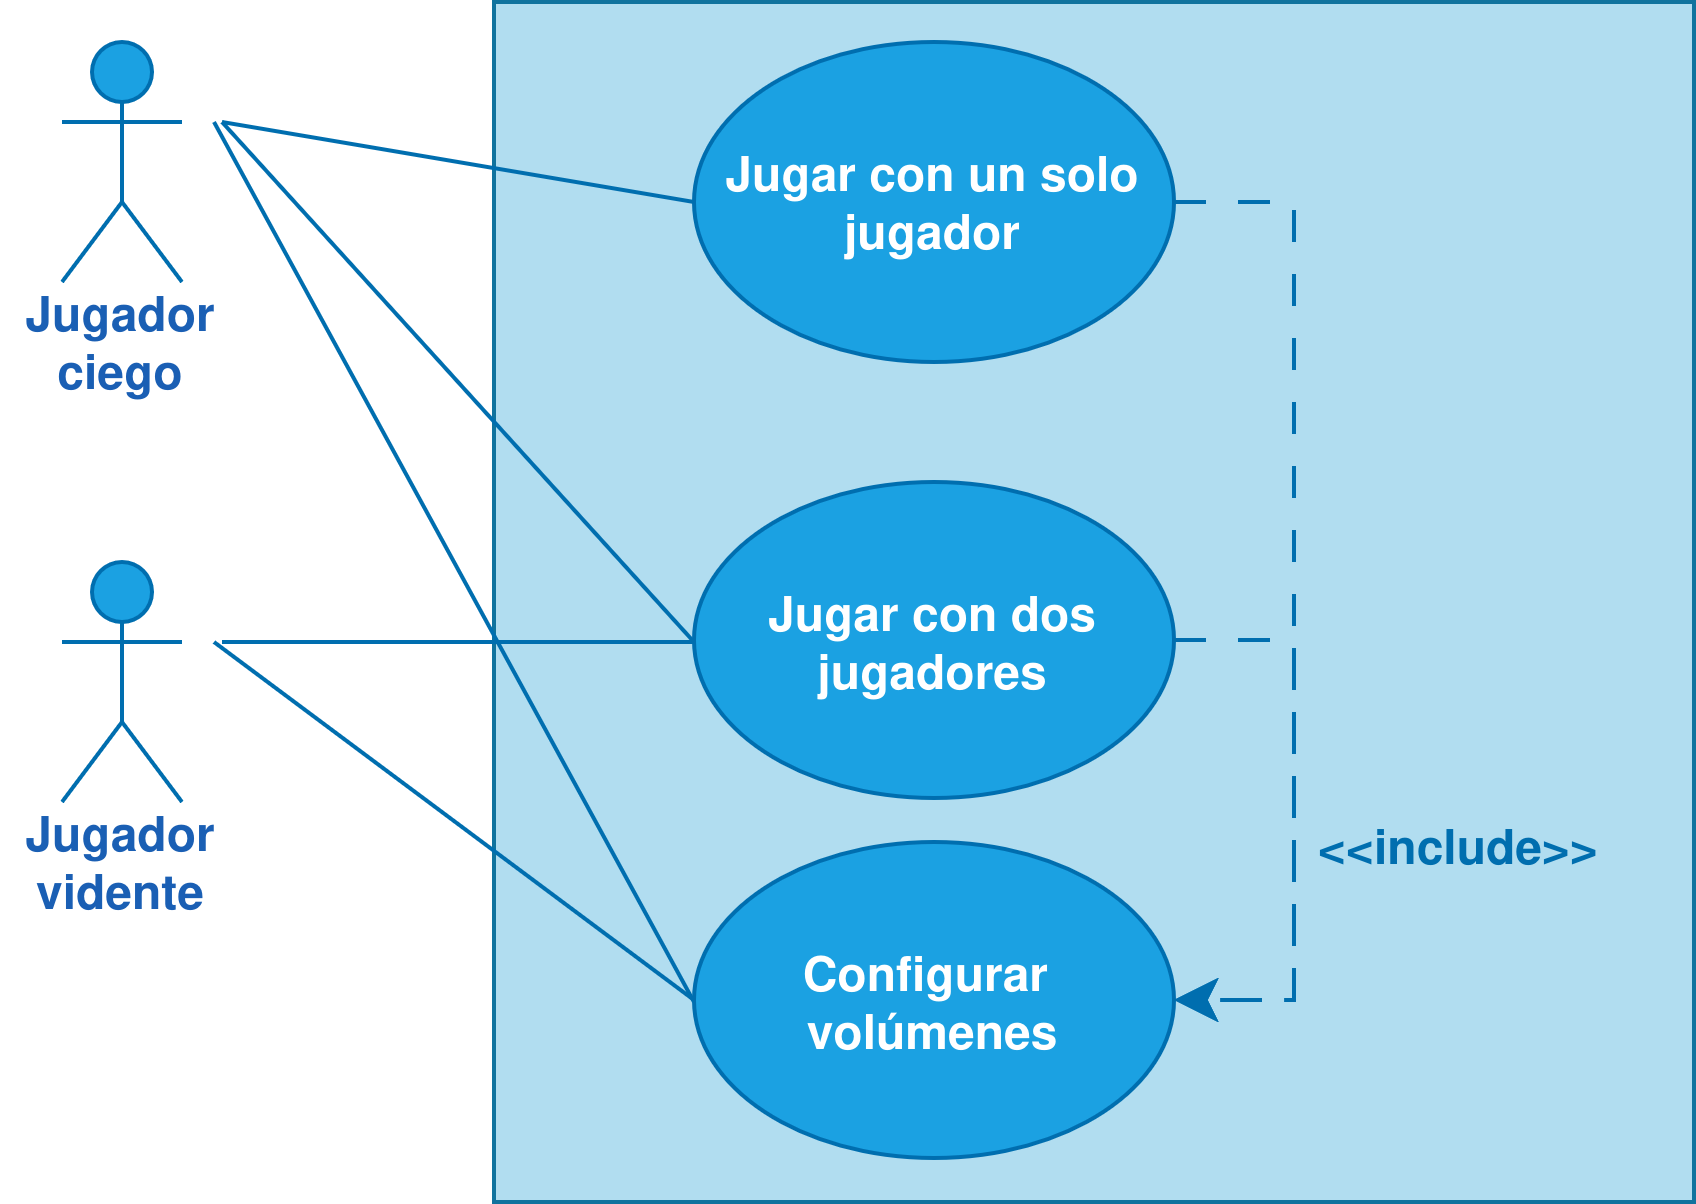
\includegraphics[width=\textwidth*2/3]{figuras/diagrama_cu.png}
		\end{adjustbox}
		
	\end{center}
	\caption{Casos de uso del juego y sus respectivos actores. Elaboración propia.}
	\label{fig:casosUso}
\end{figure}
\subsection{Escenarios de uso}
Por último, se relatan los escenarios de caso de uso en los que los actores interactúan con el juego. El proceso por el que pasan está descrito en medida de los requisitos funcionales en el diagrama de flujo de la figura \ref{fig:diagramaflujo}.
\begin{table}[H]
	\centering
	\caption{ECU-1 - Jugar con un solo jugador.}
	\label{table:ECU1}
	\begin{tabular}{|>{\centering\arraybackslash}p{6cm}|>{\centering\arraybackslash}p{8cm}|}
		\hline
		\multicolumn{2}{|c|}{\textbf{ECU-1 - Jugar con un solo jugador}} \\
		\hline
		\textbf{Actor} & \textbf{Sistema}\\
		\hline
		El jugador inicia el juego. &  \\
		\hline
		  &  El juego informa al jugador sobre los controles disponibles e inicializa los volúmenes.\\
		\hline
		 El jugador configura el sonido &  El juego almacena las preferencias de sonido del jugador y actualiza la visualización de configuración.\\
		\hline
		 El jugador selecciona el modo de juego &  El juego almacena el modo de juego y transporta al jugador al tutorial.\\
		\hline
		 &  El juego muestra tutoriales contextuales de las mecánicas del juego a medida que surgen en la partida.\\
		\hline
		El jugador utiliza el sonar o colisiona con una pared. &  El juego reproduce un sonido contextual para ayudar a la ubicación espacial del jugador.\\
		\hline
		El jugador encuentra un puzle e interactúa con él. &  El juego revisa sus variables contextuales y muestra el puzle en caso de cumplir las condiciones.\\
		\hline
		El jugador resuelve un puzle. &  El juego almacena las variables correspondientes.\\
		\hline
		El jugador resuelve todos los puzles y termina el juego. &  El juego informa auditivamente al jugador que ha terminado el juego y lo envía de nuevo al inicio.\\
		\hline
	\end{tabular}
	
\end{table}
\begin{table}[H]
	\centering
	\caption{ECU-2 - Jugar con dos jugadores.}
	\label{table:ECU2}
	\begin{tabular}{|>{\centering\arraybackslash}p{6cm}|>{\centering\arraybackslash}p{8cm}|}
		\hline
		\multicolumn{2}{|c|}{\textbf{ECU-2 - Jugar con dos jugadores}} \\
		\hline
		\textbf{Actor} & \textbf{Sistema}\\
		\hline
		Los jugadores inician el juego. &  \\
		\hline
		&  El juego informa a los jugadores visual y auditivamente sobre los controles disponibles e inicializa los volúmenes.\\
		\hline
		Los jugadores configuran el sonido &  El juego almacena las preferencias de sonido de los jugadores y actualiza la visualización de configuración.\\
		\hline
		Los jugadores seleccionan el modo de juego &  El juego almacena el modo de juego y transporta a los jugadores al tutorial.\\
		\hline
		&  El juego muestra tutoriales contextuales de las mecánicas del juego a medida que surgen en la partida.\\
		\hline
		El jugador vidente colisiona con una pared. &  El juego reproduce un sonido contextual para ayudar a la ubicación espacial del jugador ciego.\\
		\hline
		El jugador encuentra un puzle e interactúa con él. &  El juego revisa sus variables contextuales y muestra el puzle en caso de cumplir las condiciones, informa auditivamente al jugador ciego del puzle.\\
		\hline
		Los jugadores resuelven un puzle. &  El juego almacena las variables correspondientes, informa del éxito auditiva y visualmente.\\
		\hline
		Los jugadores resuelven todos los puzles y termina el juego. &  El juego informa auditivamente y visualmente a los jugadores que han terminado el juego y los envía de nuevo al inicio.\\
		\hline
	\end{tabular}
	
\end{table}

  \begin{figure}[h]

	\begin{center}
		\centering
		\begin{adjustbox}{max width=\textwidth}
			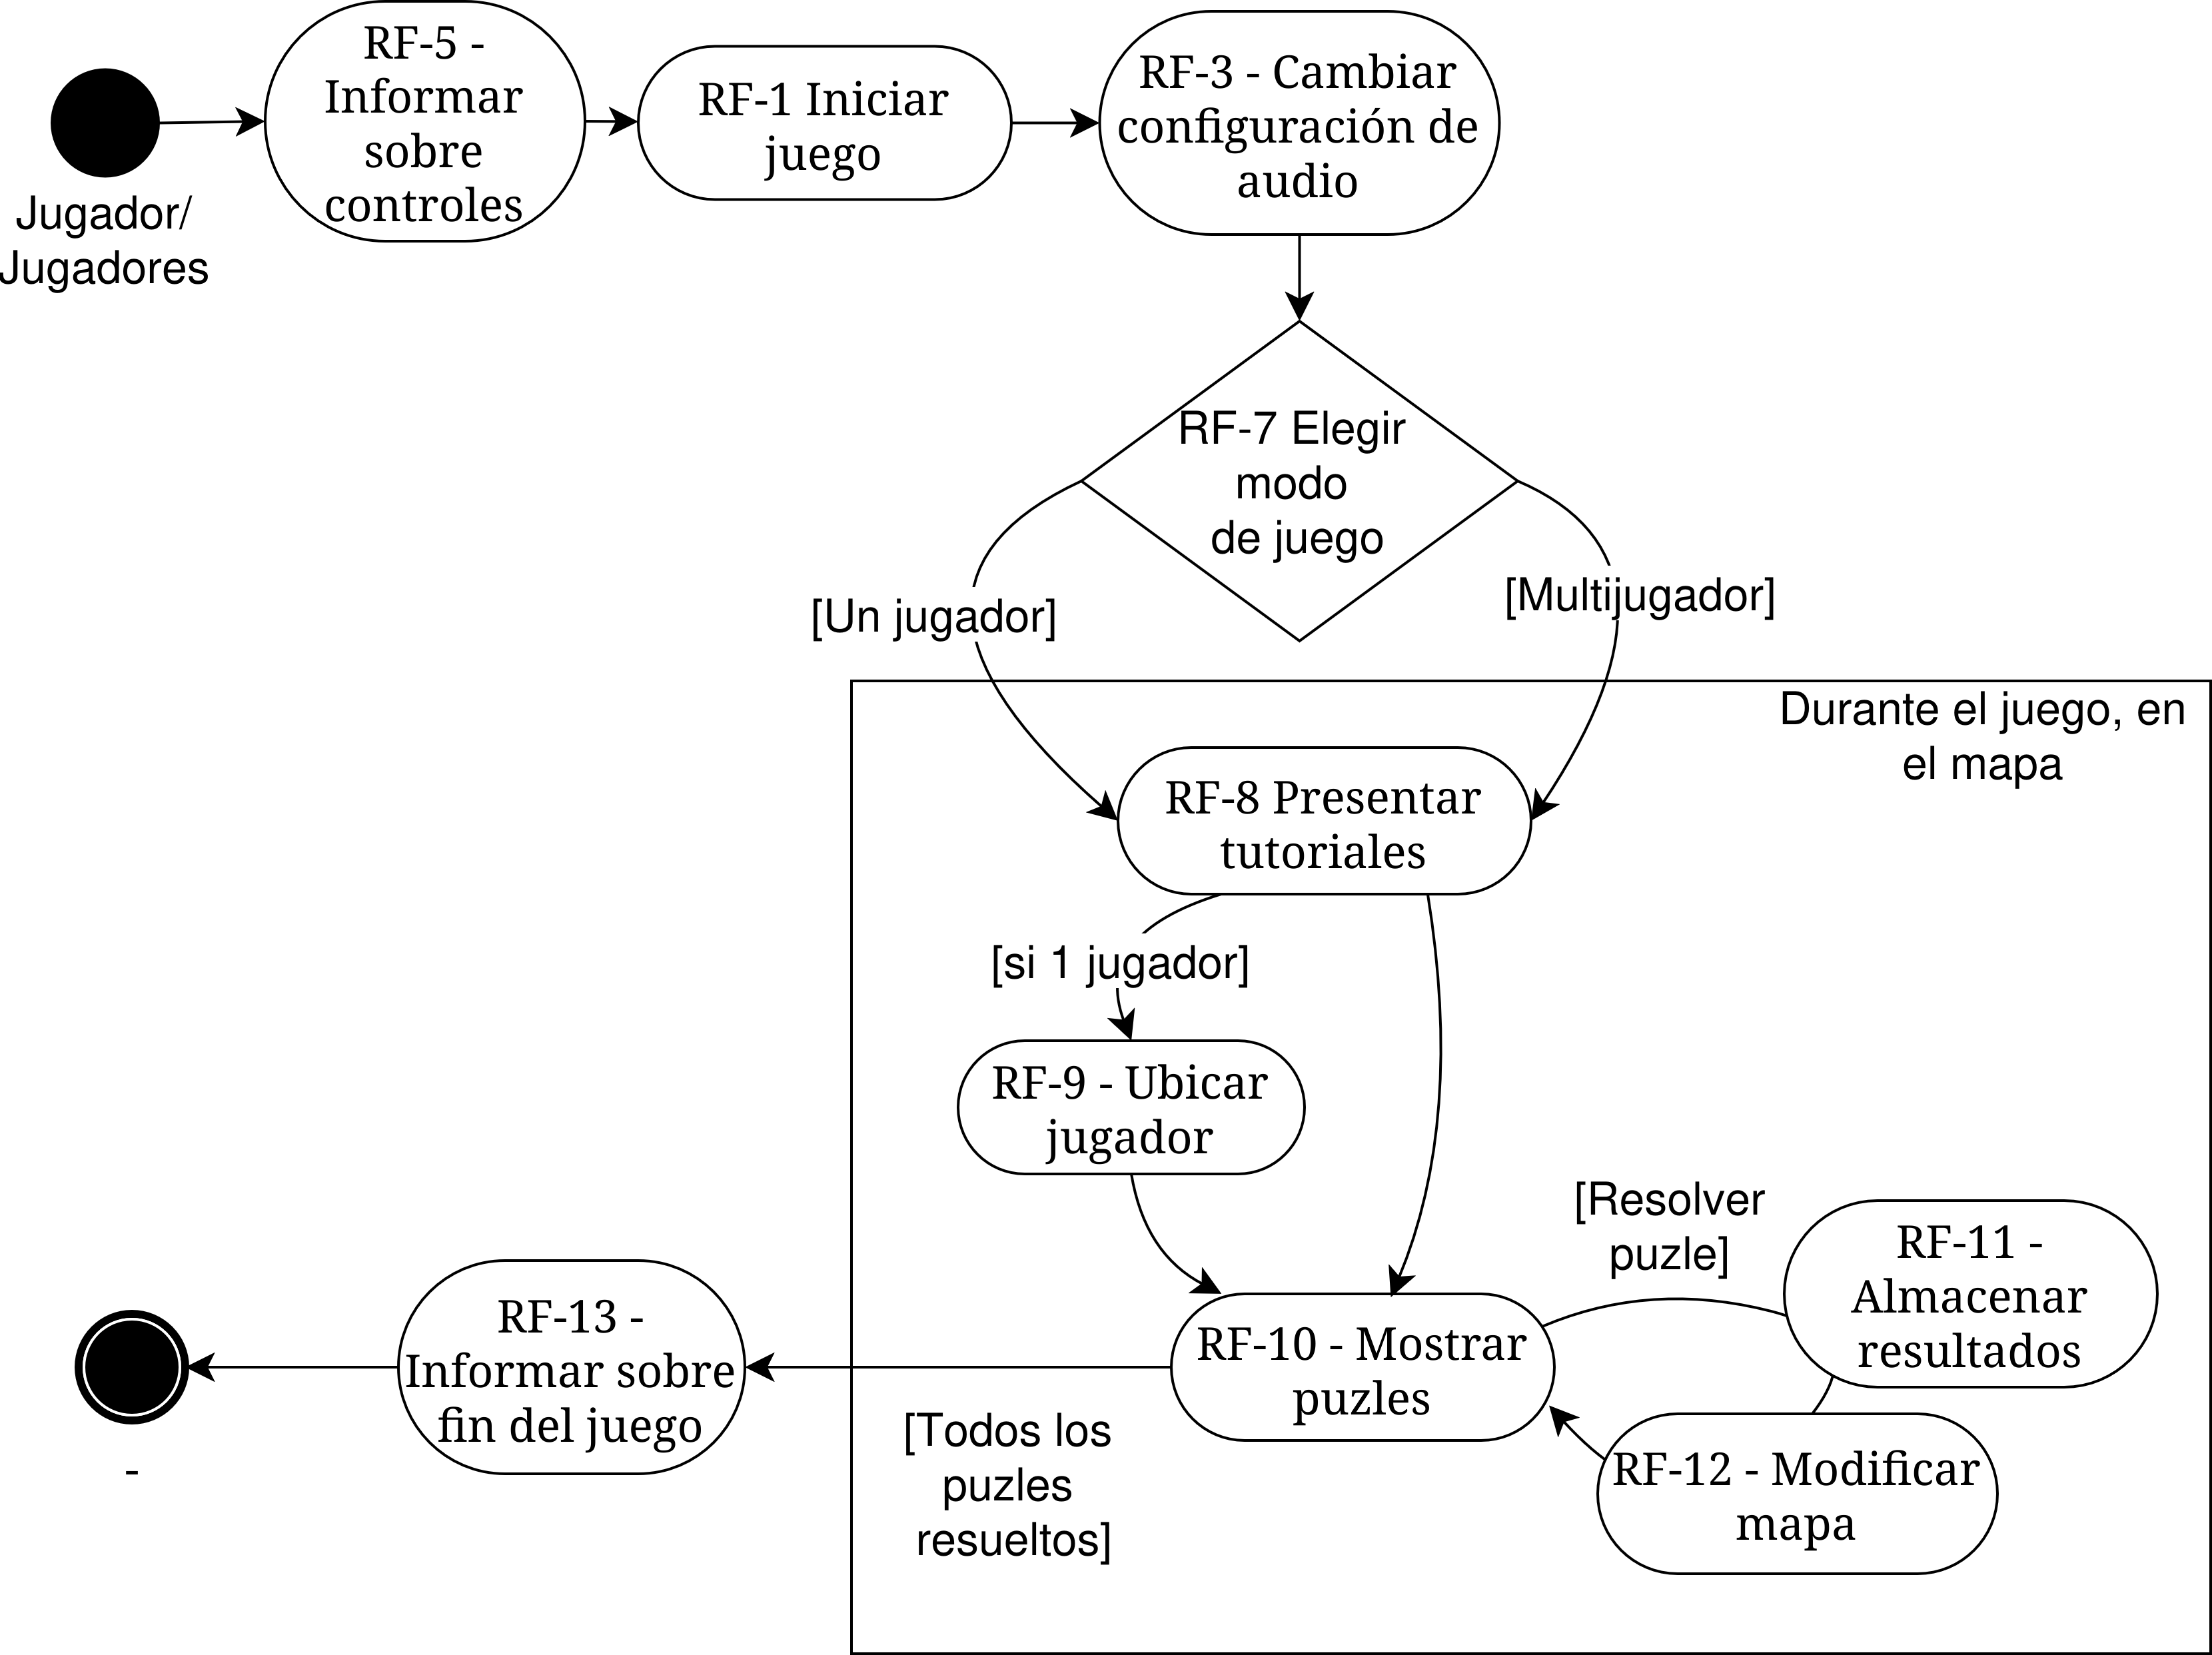
\includegraphics[width=\textwidth*3/4]{figuras/diagrama_flujo.png}
		\end{adjustbox}
		
	\end{center}
		\caption{Diagrama de flujo del juego. Elaboración propia.}
	\label{fig:diagramaflujo}
\end{figure}
\section{Planificación temporal}
% TODO redactar planificación temporal
Al inicio del trabajo, se realizó una estimación temporal que luego se evaluó a medida que se avanzó en las tareas. Para esta organización inicial, se consideraron el estado del arte, la propuesta y la redacción del resto de secciones como los tres bloques principales a los que se les debía invertir tiempo.\\

Se calcularon los días laborales, sin contar fines de semana ni festivos, para repartir las horas estimadas necesarias para un trabajo de fin de grado. Debido a la cuantía de créditos asignados a la asignatura del trabajo, se considera que la carga es de 300 horas.


\subsection{Estimación inicial}

En la estimación inicial, vista en la tabla \ref{table:EstimacionInicial}, se consideran los siguientes supuestos:
\begin{itemize}
	\item El estado del arte, junto a su redacción, ocupan un total de 47 horas y media, repartidas en 18 días laborales. Comienza el 8 de enero y termina el 27 de febrero.
	\item El desarrollo de la propuesta, junto a su redacción, toman la mayor parte de la estimación, constando de 220 horas de carga repartidas en 88 días laborales. Comienza el 28 de febrero y termina el 30 de mayo.
	\item La redacción es paralela al estado del arte y el desarrollo, pero tiene también un segmento temporal reservado exclusivamente para ella. Estos días son 15, con un total de 37 horas y media estimadas de carga. Comienza el 1 de Junio y termina el 19 de Junio.
\end{itemize}
\begin{center}
	\begin{table}[h]
		\centering
		\caption{Estimación temporal inicial de la carga de trabajo.}
		\label{table:EstimacionInicial}
		\begin{adjustbox}{max width=\textwidth}
			\begin{NiceTabular}{ |>{\centering\arraybackslash}c|>{\centering\arraybackslash}c|>{\centering\arraybackslash}c|>{\centering\arraybackslash}c|>{\centering\arraybackslash}c|>{\centering\arraybackslash}c|>{\centering\arraybackslash}c| }
				\midrule
				\textbf{Tarea} & Enero & Febrero & Marzo & Abril & Mayo & Junio \\	
				\midrule
				Estado del arte & \cellcolor{blue} & \cellcolor{blue}  &  &  &  &  \\
				\midrule
				Propuesta & & & \cellcolor{red} & \cellcolor{red} & \cellcolor{red} &  \\
				\midrule
				Redacción & \cellcolor{yellow} & \cellcolor{yellow}  & \cellcolor{yellow} & \cellcolor{yellow} & \cellcolor{yellow} & \cellcolor{yellow} \\
				\midrule
			\end{NiceTabular}
		\end{adjustbox}
	\end{table}
\end{center}
\subsection{Estimación pesimista}
La estimación inicial considera que las predicciones de fechas y horarios se siguen sin incidencias. Considera reuniones con el tutor y aprendizaje de herramientas. En caso de que hubiera imprevistos que atrasaran severamente las secciones, se realiza una estimación pesimista, resumida en la tabla \ref{table:EstimacionPesimista}:
\begin{itemize}
	\item El estado del arte toma 28 días, 70 horas. Inicia el 8 de enero y termina el 20 de marzo.
	\item El desarrollo de la propuesta, retrasado por la redacción del estado del arte, inicia el 21 de marzo, finaliza el 14 de junio. Toma 89 días, 222 horas.
	\item La redacción es paralela al estado del arte y el desarrollo y finaliza el 19 de junio, como en la anterior estimación.
\end{itemize}
\begin{center}
	\begin{table}[h]
		\centering
		\caption{Estimación temporal pesimista de la carga de trabajo.}
		\label{table:EstimacionPesimista}
		\begin{adjustbox}{max width=\textwidth}
			\begin{NiceTabular}{ |>{\centering\arraybackslash}c|>{\centering\arraybackslash}c|>{\centering\arraybackslash}c|>{\centering\arraybackslash}c|>{\centering\arraybackslash}c|>{\centering\arraybackslash}c|>{\centering\arraybackslash}c| }
				\midrule
				\textbf{Tarea} & Enero & Febrero & Marzo & Abril & Mayo & Junio \\	
				\midrule
				Estado del arte & \cellcolor{blue} & \cellcolor{blue}  & \cellcolor{blue}  &  &  &  \\
				\midrule
				Propuesta & & &  & \cellcolor{red} & \cellcolor{red} & \cellcolor{red} \\
				\midrule
				Redacción & \cellcolor{yellow} & \cellcolor{yellow}  & \cellcolor{yellow} & \cellcolor{yellow} & \cellcolor{yellow} & \cellcolor{yellow} \\
				\midrule
			\end{NiceTabular}
		\end{adjustbox}
	\end{table}
\end{center}
\subsection{Estimación optimista}
En caso de que se le invirtiera más tiempo inicialmente al estado del arte, considerando que en los meses de enero el tiempo disponible es mayor, resulta en la estimación optimista. Se crea bajo la suposición de que los días laborales son de una duración variable, a diferencia de las 2.5 horas fijas de las anteriores estimaciones. Tal y como se muestra en la tabla \ref{table:EstimacionOptimista}:

\begin{itemize}
	\item El estado del arte toma 11 días, 47 horas. Inicia el 8 de enero y termina el 15 febrero.
	\item El desarrollo de la propuesta, inicia el 16 de febrero, finaliza el 17 de mayo. 
	\item La redacción finaliza el 3 de junio, al comenzar temprano.
\end{itemize}
\begin{center}
	\begin{table}[h]
		\centering
		\caption{Estimación temporal optimista de la carga de trabajo.}
		\label{table:EstimacionOptimista}
		\begin{adjustbox}{max width=\textwidth}
			\begin{NiceTabular}{ |>{\centering\arraybackslash}c|>{\centering\arraybackslash}c|>{\centering\arraybackslash}c|>{\centering\arraybackslash}c|>{\centering\arraybackslash}c|>{\centering\arraybackslash}c|>{\centering\arraybackslash}c| }
				\midrule
				\textbf{Tarea} & Enero & Febrero & Marzo & Abril & Mayo & Junio \\	
				\midrule
				Estado del arte & \cellcolor{blue} & \cellcolor{blue}  &  &  &  &  \\
				\midrule
				Propuesta & & & \cellcolor{red} & \cellcolor{red} & \cellcolor{red} &  \\
				\midrule
				Redacción & \cellcolor{yellow} & \cellcolor{yellow}  & \cellcolor{yellow} & \cellcolor{yellow} & \cellcolor{yellow} &  \\
				\midrule
			\end{NiceTabular}
		\end{adjustbox}
	\end{table}
\end{center}
\subsubsection{Justificación de las estimaciones y estimación final}
En la estimación optimista se reduce el tiempo invertido en el estado del arte debido a que es el periodo con menor carga académica al coincidir con el inicio del semestre. Además, el estado del arte se considera finito y determinable, es decir, cuando se justifican correctamente las decisiones tomadas en el trabajo y se explora con suficiente profundidad el área de estudio, se finaliza. Debido a la variabilidad del desarrollo, se confía menos en reducir su carga horaria. \\

La estimación final se realiza mediante una estimación multipunto \cite{projectmanagementinstituteGuideProjectManagement2017}. Es una media entre la estimación optimista, pesimista y más probable cuando hay incertidumbre:
\[
	T_E = (T_O + T_M + T_P)/3
\]
Siendo $T_E$ la estimación esperada, $T_O$ la estimación optimista, $T_M$ la estimación más probable y $T_P$ la pesimista.
Esta estimación resulta en las siguientes fechas:
\begin{itemize}
	\item El estado del arte toma 19 días, 48 horas. Inicia el 8 de enero y termina el 2 de marzo.
	\item El desarrollo de la propuesta, inicia el 3 de marzo, finaliza el 31 de mayo. 
	\item La redacción empieza el 2 de junio y finaliza el 14 de junio.
\end{itemize}
\subsubsection{Reevaluación de la estimación en desarrollo}
A medida que se redactaron las subsecciones del estado del arte, la evaluación temporal se acercó más a la estimación pesimista, puesto que esta parte acabó el 19 de Marzo, mucho después de las estimaciones previstas como más probable y final. \\

En cuanto al desarrollo, se empezó la programación el 20 de Marzo y se terminó el primer prototipo el 29 de Marzo. La versión completa del desarrollo fue finalizada el 28 de Mayo, coincidiendo con la estimación inicial. Sin embargo, se realizó un parche del prototipo el 4 de Junio para facilitar las pruebas de usuario.\\

Durante el desarrollo, se concertó un periodo de pruebas de usuario con el proyecto Modos-ON de la ONCE, lo cual requirió invertir tiempo de desarrollo y redacción en reuniones y prototipado adicional para asegurar que el trabajo cumplía todos los requisitos necesarios. Por último, el periodo reservado a la redacción comenzó el 5 de junio. \\

Tras finalizar el proyecto, se obtuvo una cantidad de horas total de 317. Las estimaciones están representadas en un diagrama de Gantt en la figura \ref{fig:gantt}. La planificación final de horas con los tiempos reales se lista a continuación:
\begin{enumerate}

\item\textbf{Redacción y desarrollo del estado del arte}
\subitem a.  Se organizaron las distintas fases del trabajo y se estimó la duración inicial de las tareas. Se investigaron la legislación y los estándares disponibles para el desarrollo de audiojuegos accesibles.
\subitem b. Tareas implicadas:
\subsubitem i. Definición del alcance del estado del arte y sus secciones. Del 13 de enero al 15 de enero.
\subsubitem ii. Comparativa de herramientas de desarrollo e investigación. Del 8 de enero al 12 de enero.
\subsubitem iii. Selección de herramientas para la revisión. Del 12 enero a 13 de enero.
\subsubitem iv Revisión de la legislación. Del 21 febrero al 2 de marzo.
\subsubitem v. Redacción de Heurísticas. Del 2 marzo a 19 de marzo.
\subsubitem vi. Estudio de audiojuegos. Del 13 enero al 20 febrero.
\subitem c. Tiempo real: 105.5 horas.
\item \textbf{Desarrollo del juego}
\subitem a. Se realizó un análisis de los requisitos funcionales, no funcionales y de información. Se diseñó y desarrolló un prototipo inicial del audiojuego.
\subitem b. Tareas implicadas:
\subsubitem i. Especificación de requisitos y casos de uso. Del 20 marzo al 22 de marzo.
\subsubitem ii. Reuniones semanales con el tutor del trabajo. Del 15 de enero hasta 16 de junio.
\subsubitem iii. Diseño inicial de las pruebas de usuario. Del 28 mayo al 4 junio.
\subsubitem iv. Diseño de los puzles sonificados. Del 6 de abril al 18 de mayo.
\subsubitem v. Diseño de las interfaces. Del 22 de marzo al 31 de marzo.
\subsubitem vi. Pruebas de desarrollo. Del 26 de mayo al 11 de junio.
\subitem c. Tiempo real: 183.5 horas.
\item \textbf{Pruebas de usuario y finalización de memoria}
\subitem a. Se consultaron a usuarios finales y expertos para mejorar la aplicación desarrollada. Se redactaron los últimos detalles del trabajo.
\subitem b. Tareas implicadas:
\subsubitem i. Definición de un cuestionario de calidad. Del 25 al 26 de mayo.
\subsubitem ii. Modificaciones del prototipo para ajustarse al \textit{feedback}. Del 1 de junio al 5 de junio.
\subsubitem iii. Reuniones con los usuarios para consultar sus dudas y sugerencias. Del 25 de mayo al 3 junio.
\subitem c. Tiempo real: 28 horas.
\end{enumerate}
  \begin{figure}[h]
	\centering
	\begin{adjustbox}{max width=\textwidth}
		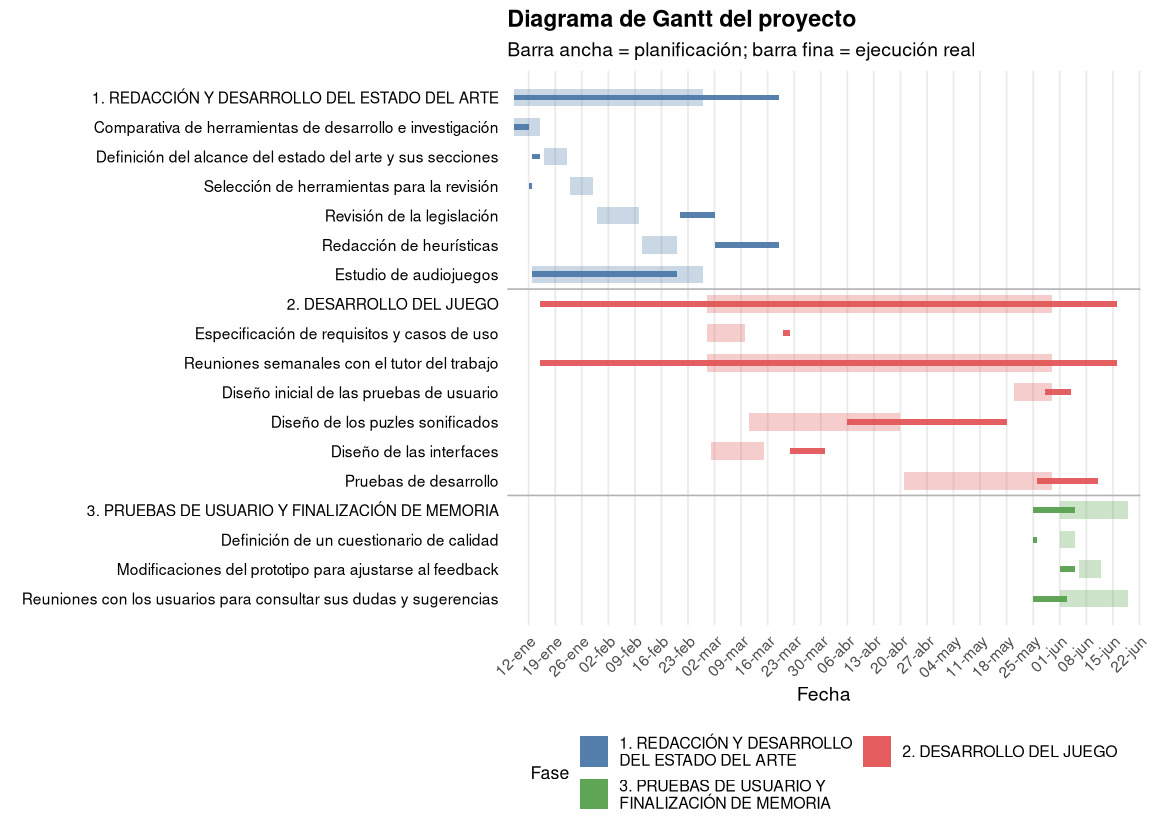
\includegraphics[width=\textwidth]{figuras/diagrama_gantt.jpeg}
	\end{adjustbox}
	\caption{Diagrama de gantt de las tareas con su estimación y el tiempo real. Elaboración propia.}
	\label{fig:gantt}
\end{figure}
\section{Costes y presupuesto}
% TODO redactar costes y presupuesto
En esta sección se estimará el coste aproximado del proyecto en su conjunto dividido en secciones según los tipos de gastos que se han considerado.


\subsection{Costes de personal}

 Se considera que el desarrollador de software junior ha invertido, asumiendo tanto la etapa de análisis e investigación como el desarrollo, un total de 317 horas laborales. El tutor, por su parte, se considera en la sección de planificación y diseño del trabajo, constando en su presupuesto 25 horas laborales.\\

Según el Régimen General de la Seguridad Social, particularmente en la \textit{Orden PJC/297/2026, de 30 de marzo} \cite{ministeriodelapresidenciajusticiayrelacionesconlascortesOrdenPJC2972026}, las bases de cotización de los ingenieros técnicos oscilan entre un mínimo de 1.649,70 \euro y un máximo de 5.101,20 \euro mensuales. Asumiendo que estos límites se calculan sobre un horario de trabajo a tiempo completo, se obtienen los siguientes sueldos por hora:\\
\[
\frac{1.649,70 \euro}{40 \text{h} \cdot 4  \text{ semanas}} \approx 10,31 \euro / \text{hora}
\]
\[
\frac{5.101,20 \euro}{40 \text{h} \cdot 4  \text{ semanas}} \approx 31,88 \euro / \text{hora}
\]

Estimando la media de ambas,

\[
\frac{31,88\euro + 10,31\euro}{2} = 21,095\euro
\]

y multiplicándolo por las horas invertidas obtenemos un total de 

\[
	21,095\euro \cdot 317\text{h} \approx 6687,12 \euro
\]
 Por otro lado, para estimar los costes asociados a las horas del tutor, tomamos de referencia las retribuciones del PDI de la Universidad de Granada \cite{ServicioHabilitacionSeguridad} y asumimos una media de 31,38 \euro / hora. 
\[ 
 	31,38\euro \cdot 25\text{h} \approx 784,5 \euro
\]

El coste total de personal suma 7471,62 \euro, se asume que el IRPF está incluido y se reduce del total una vez se paguen los salarios.
 
\subsection{Costes indirectos}
Se consideran costes indirectos los implicados en infraestructura para soportar el día a día del desarrollador. En estos costes contabilizamos agua, luz, conexión a internet, comida y alquiler. Para un periodo estimado desde enero de 2026 hasta junio, se consideran estos gastos un total de:
\[ 
	850\euro \cdot 6 \text{ meses} = 5100\euro
\]
\subsection{Costes de material}
Respecto a las licencias necesarias para el desarrollo de este proyecto, se han utilizado herramientas de código abierto con el fin de reducir costes y facilitar la distribución. El motor de desarrollo principal ha sido Godot, junto a su lenguaje propio Gdscript, que no requieren de costes. \\

Con el fin de calcular el coste del \textit{hardware} utilizado en el proyecto, se asume el precio original del portátil empleado para la programación (1110\euro)  y una vida útil de 6 años:

\[
1110 \euro / 6 \text{ años} = 185 \euro /\text{año}
\]
Como el proyecto se desarrolla en un periodo de 6 meses, el coste total de materiales es 92,5\euro.
\subsection{Coste total}
Contabilizando todos los costes implicados en el desarrollo del trabajo, se muestra en la tabla \ref{table:Presupuesto del proyecto} a modo resumen del presupuesto total.

\begin{table}[H]
	\centering
	\caption{Coste total del proyecto.}
	\label{table:Presupuesto del proyecto}
	\begin{tabular}{|l|c|}
		\hline
		\textbf{Sección}  & \textbf{Coste por 6 meses (\euro)}\\
		\hline
		Coste de personal & 7471,62 \\
		Costes indirectos & 5100 \\
	Costes de material & 92,5 \\
	\textbf{Coste total} & 12664,12 \\
		\hline
	\end{tabular}
	
\end{table}
\section{Plan de gestión de riesgos}
Los riesgos posibles en un audiojuego dependen del propósito que tenga. En cuestiones económicas, en caso de ser publicado por un estudio de videojuegos con el objetivo de recuperar los costes de desarrollo y conseguir un beneficio, existe el riesgo de que la inversión no se recupere y los desarrolladores pierdan dinero. Como este trabajo no pretende ser publicado en una plataforma de monetización de videojuegos, ese riesgo no se considera.\\

En cuestiones de almacenamiento y catástrofes electrónicas, como apagones de luz, averías y roturas, se tiene en mantenimiento y actualización una copia de los datos en plataformas de gestión de archivos en la nube y en diferentes dispositivos.\\

Este trabajo no utiliza servidores para ninguna de sus funcionalidades y por lo tanto no sufre de caídas de servicio ni requiere de capas de ciberseguridad adicionales.\\

Respecto a las tecnologías utilizadas, el uso de una tecnología y las horas invertidas en ella pueden llegar a resultar infructíferas, perdiendo así horas destinadas al desarrollo. Esto es natural y esperado y se considera en las horas destinadas a la propuesta en la estimación temporal. Para evitarlo, se revisan minuciosamente las alternativas disponibles antes de decidir cuál es la más apropiada para el trabajo.\\

Por último, existe el riesgo del retraso respecto a la estimación final temporal. Este riesgo es asumido y esperable, tanto por la falta de experiencia en la realización de estas estimaciones como por el desconocimiento de los posibles desafíos de desarrollo. Las estimaciones son todas asumibles, incluso la pesimista, para entregar el trabajo en las fechas previstas por la convocatoria ordinaria y las estimaciones sirven como un marco al que aspirar en organización y metas.\\

\section{Desarrollo}
%TODO redactar desarrollo
En esta sección, se describirán las herramientas seleccionadas para el desarrollo del trabajo, las fases de prototipado seguidas y las pruebas de usuario realizadas.

\subsection{Herramientas de desarrollo}
Para el desarrollo del juego se realizó un estudio comparativo de algunas herramientas de desarrollo de videojuegos con el fin de elegir la más adecuada. Se consideraron los siguientes criterios:
\begin{itemize}
	\item Disponibilidad para Linux, al ser el sistema operativo principal de la desarrolladora.
	\item Precio. Se favorecen herramientas gratuitas para reducir costes.
	\item Licencia. Necesariamente las herramientas deben presentar una licencia libre para cumplir el Requisito no funcional RNF-5 presente en la tabla \ref{table:RNF}.
	\item Herramientas de accesibilidad. Compatibilidad con el lector de pantallas del sistema y modos de enfoque de interfaces compatibles con sistemas operativos adaptados.
	\item Sistemas de gestión de audio posicional. Una de las herramientas principales del juego es el audio, a través del cual se representa la información de las interfaces y los objetos. El motor seleccionado debe presentar esta característica.
	\item Motor de videojuegos. La herramienta seleccionada debe ser un motor de videojuegos, para emular el estándar en la industria. Esto  se debe a la diversidad profesional de los equipos que los usan (personal de audio, gráficos, diseñadores y programadores).
	\item Tiempo de desarrollo. La herramienta debe tener un desarrollo activo, una documentación actualizada y ser considerada estable para su utilización en el proyecto.
\end{itemize}
\begin{center}
	\begin{table}[h]
		\centering
		\caption{Comparativa de herramientas de desarrollo.}
		\label{table:comp-engines}
		\begin{adjustbox}{max width=\textwidth}
			\begin{NiceTabular}{ |>{\centering\arraybackslash}m{3.3cm}||>{\centering\arraybackslash}m{3cm}|>{\centering\arraybackslash}m{3cm}|>{\centering\arraybackslash}m{3cm}|>{\centering\arraybackslash}m{3cm}|>{\centering\arraybackslash}m{3cm}|>{\centering\arraybackslash}m{3cm}|  }
				
				\midrule
				\textbf{Criterio} \textbackslash \textbf{Motor} & \textbf{Unreal Engine} & \textbf{Unity} & \textbf{CryEngine} & \textbf{GameMaker} & \textbf{Godot Engine} & \textbf{Panda3D}\\
				\midrule[1pt]
				\textbf{Disponibilidad para Linux} & No & Sí  &  No & Sí (en beta) & Sí & Sí \\
				\midrule
				\textbf{Precio} & Gratis, pagas regalías & Gratis, planes de pago para empresas &  Gratis, pagas regalías & De Pago & Gratis & Gratis \\
				\midrule
				\textbf{Licencia} & Propietaria (con código fuente disponible) & Propietaria  &  Propietaria & Propietaria & MIT (Libre) & BSD (Libre) \\
				\midrule
				\textbf{Herramientas de accesibilidad} & Integración experimental con lectores de pantalla. & Múltiples \textit{plugins} de la comunidad.  &  Pocas herramientas dedicadas & No & Lector de pantallas experimental & No \\
				\midrule
				\textbf{Audio posicional} & Sí & Sí  &  Sí & Reducido & Sí & Sí \\
				\midrule
				\textbf{Desarrollo / Última versión estable} & En desarrollo activo & En desarrollo activo  &  En desarrollo, última versión antigua  & En desarrollo activo & En desarrollo activo & En desarrollo activo \\
				\midrule
			\end{NiceTabular}
		\end{adjustbox}
	\end{table}
\end{center}
Debido a su reciente inclusión de herramientas de accesibilidad \cite{engine_dev_nodate}, su desarrollo activo, la disponibilidad de documentación en línea, su gratuidad y la licencia libre MIT, finalmente se decidió utilizar Godot para este trabajo.
\subsection{Metodologías de desarrollo}
Para este trabajo se siguió una metodología de prototipado cíclica semanal. En la primera iteración se creó un juego base sobre el que se fueron construyendo semanalmente características definidas en reuniones fijas con el tutor. Si las características requerían de una iteración adicional, se consideraba en la reunión y se reajustaban las estimaciones posteriores. Este modelo de desarrollo permitió su adaptación posterior a las pruebas de usuario, considerando las modificaciones requeridas como tareas incluidas en las iteraciones.
\subsection{Análisis}
% 1. Análisis de requisitos
	% 2. Análisis de las soluciones
	% 3. Solucion propuesta
	% 4. Análisis de seguridad
En el desarrollo de la aplicación se encontraron desafíos relacionados al ejercicio de abstracción necesario para considerar las interfaces convencionales de un videojuego y trasladarlas a un audiojuego accesible. Ya que el juego se diseña para ser jugado por una sola persona o dos en cooperación, es necesario diseñar dos veces cada puzle implementado. En el primer diseño, se considera el puzle completamente sonificado, para obviar la interfaz gráfica en caso de que el jugador tenga discapacidad visual total. En el segundo diseño, se considera que uno de los jugadores debe tener en cuenta la interfaz gráfica y otro la auditiva, así que ambos componentes son necesarios para resolver los retos planteados. La distinción de estas dos metodologías de diseño repercutió en el desarrollo y exigió la duplicación y modificación de los escenarios programados. \\

Al tenerse en cuenta la presencia de un jugador sin discapacidad visual, se obvia el mecanismo de ubicación por el mapa por sonar necesario en la modalidad de un solo jugador. A cambio, los puzles deben complejizarse para favorecer el trabajo en grupo y no permitir que ninguno de los dos jugadores considere que su papel es secundario.\\

Uno de los mayores retos del diseño de estos juegos fue priorizar controles sencillos y simplificados. Se tuvo como objetivo que todo el juego pudiera controlarse con un botón de interacción, un botón de sonar y las flechas de movimiento. De esta forma se reduce la confusión que los controles complejos pudieran añadir a la jugabilidad y se pueden analizar mejor las estrategias empleadas.\\
\subsection{Implementación}
El desarrollo se realizó a través de iteraciones jugables completas que implementaban los requisitos del juego en niveles de prioridad.
\subsubsection{Primera iteración}
En la primera iteración se aspiraba a obtener un producto jugable, completo, que implementara heurísticas de accesibilidad visual y que se pudiera terminar sin requerir el uso de una interfaz gráfica.
Debido a que la interfaz gráfica es obviable, en este caso se utilizaron \textit{placeholders} para la composición del nivel y la ilustración que representa al jugador en movimiento. El primer requisito esencial que se desarrolló fue el uso de \textit{TTS (Text To Speech)} a través del Sistema Operativo para sonificar las interfaces de los menús. También se aseguró que el foco de los botones funcionara correctamente solo con el teclado. Se crearon preferencias de usuario relacionadas con los diferentes sonidos que se utilizan en el juego y se proporcionaron los medios para otorgar voces distintas a los menús y a las acciones, para diferenciar correctamente lo que realiza el jugador en cada momento.\\

En cuanto al audiojuego, se creó un puzle auditivo compuesto por una melodía que había que recordar y reproducir en otro punto del mapa a través de botones. También se incluyó la opción de ubicarse en el mapa a través del sonar, que se sonificó modificando el timbre y el eco de un sonido respecto a la posición del jugador.\\

En esta primera iteración se demostraron las técnicas de sonificación investigadas en la sección de estado del arte y se aplicaron a un entorno interactivo para probar su funcionalidad.\\
\subsubsection{Segunda iteración}
Posteriormente, se incluyó la modalidad de multijugador. La elección de este modo de juego se considera como parte de las interfaces de inicio y se almacena como una variable global para su posterior consulta en el juego. El diseño de los mapas es el mismo para ambas modalidades, los objetos con los que los jugadores interactúan y los textos descriptivos que informan sobre el contexto se modifican en base a si son dos jugadores o uno.\\

Además, en esta iteración comenzó el diseño de un tutorial introductorio que explica las mecánicas básicas al jugador a medida que utiliza el juego. En este tutorial, se presenta un mapa muy reducido con pocas zonas de interacción, para favorecer que los jugadores aprendan jugando. Se creó un objeto (fusible) que se debía encontrar explorando la sala y se debía utilizar en otro (robot/artefacto) para desbloquear el sonar y poder acceder al mapa principal. \\

En esta iteración se necesitó duplicar los tutoriales tanto en interfaces, puesto que el jugador vidente debía tener un menú con los controles y el jugador ciego un sonido explicativo, como en modo de juego. Por último, se incluyó el soporte de mando. \\

\subsubsection{Tercera iteración}
En la siguiente iteración, se diseñó el mapa final del juego, donde se situarían todos los minijuegos disponibles posteriores al tutorial. El mapa que se creó en esta sección está representado en la figura \ref{fig:mapa_juego} para su posterior referencia. \\

  \begin{figure}[h]
		\centering
		\begin{adjustbox}{max width=\textwidth}
			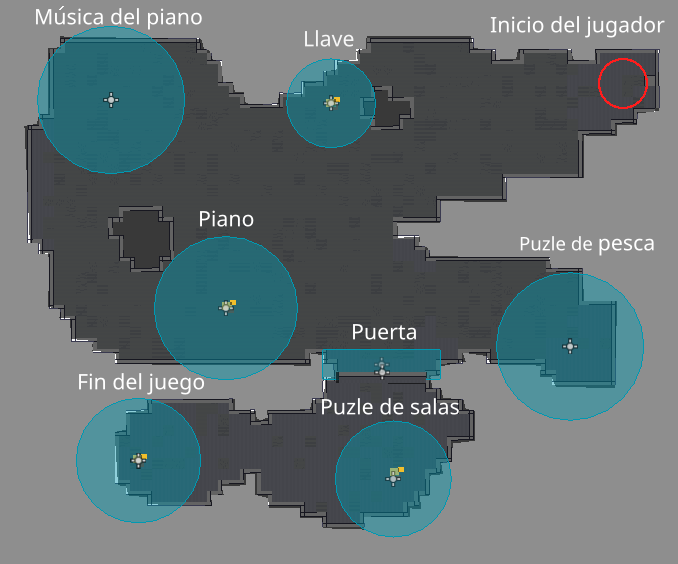
\includegraphics[width=\textwidth*3/4]{figuras/mapa_juego.png}
		\end{adjustbox}
	\caption{Mapa del juego y ubicación de los puzles sonificados. Elaboración propia.}
	\label{fig:mapa_juego}
\end{figure}
Las áreas azules de esta imagen representan las zonas en las que los jugadores pueden interactuar con los elementos que representan. Son más grandes que en un juego convencional para facilitar la jugabilidad. El propósito de estas áreas es compensar la dificultad de navegación que supone la ausencia de visión permitiendo encontrar los objetos clave con mayor rapidez y volver a ubicarlos sin depender de precisión visual.\\

\subsubsection{Cuarta iteración}
Posterior al diseño del mapa, se concluyó un minijuego empezado en la anterior iteración y se diseñó otro adicional en las semanas subsecuentes. \\

El primer minijuego es el puzle de pesca. El diseño de este reto está basado en una mecánica popular en los videojuegos comerciales que consiste en reaccionar rápidamente a un signo visual que indica que un pez ha picado el anzuelo. La dificultad del diseño de este juego consiste en integrar todas las señales en una única interfaz auditiva y, para la versión de multijugador, ajustar los tiempos para que la comunicación entre los jugadores sea suficiente para resolverlo. Además fue necesario incluir voces contextuales que explicaran los estados de fracaso y éxito ya que no se podía utilizar una señal visual y los sonidos de efecto no eran suficientes por sí mismos. \\

Por otro lado, se imitó la mecánica del tutorial y se añadió un objeto en la parte superior del mapa que desbloqueaba la zona inferior. De esta forma, se busca incentivar la exploración y añadir estímulos al jugador en zonas que, sin este objeto, serían demasiado extensas sin estímulo, favoreciendo la confusión de orientación. Los textos descriptivos de la puerta se modificaban en base a si se había conseguido o no la llave.\\
\subsubsection{Quinta iteración}
Tras una reevaluación de la jugabilidad, se consideró oportuno desarrollar un sistema de sombras que dificultara en mayor medida la visión del jugador vidente en el modo multijugador. Esto se basa en la hipótesis de que, al reducir su capacidad de orientación, dependería más del jugador ciego, que obtiene información a través de sonidos. La efectividad de esta mecánica estaba diseñada para comprobarse en las pruebas de usuario. \\

Se incluyó un puzle sonificado adicional, diseñado para hacer una asociación entre los sonidos ambientales que se podían escuchar en una sala con las descripciones de las baldosas en las tres direcciones disponibles para avanzar. Este puzle trata de imitar otro desafío común en videojuegos, un laberinto. En los juegos tradicionales, se necesita de una pista previa o de la observación de elementos presentes en el mapa para elegir correctamente la dirección. Como no es posible depender de una interfaz visual completa, se opta por diseñar dos versiones según el modo de juego. \\
  \begin{figure}[h]
	\centering
	\begin{minipage}[b]{0.4\textwidth}
		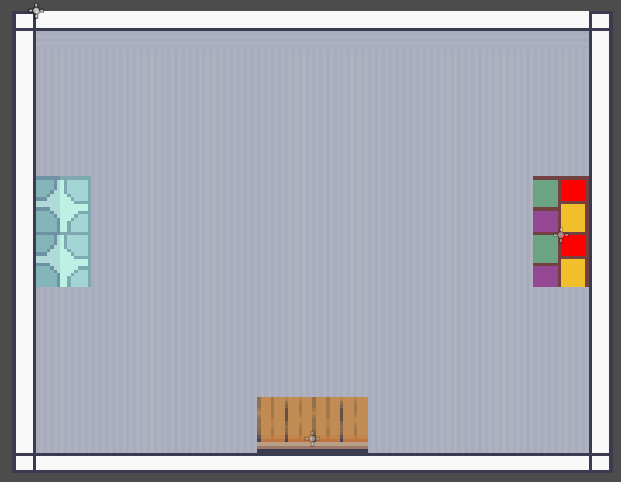
\includegraphics[width=\textwidth]{figuras/mapa_salas_mul.png}
		\caption{Puzle de salas en su versión multijugador.}
		\label{fig:mapa_salas_mul}
	\end{minipage}
	\hfill
	\begin{minipage}[b]{0.4\textwidth}
		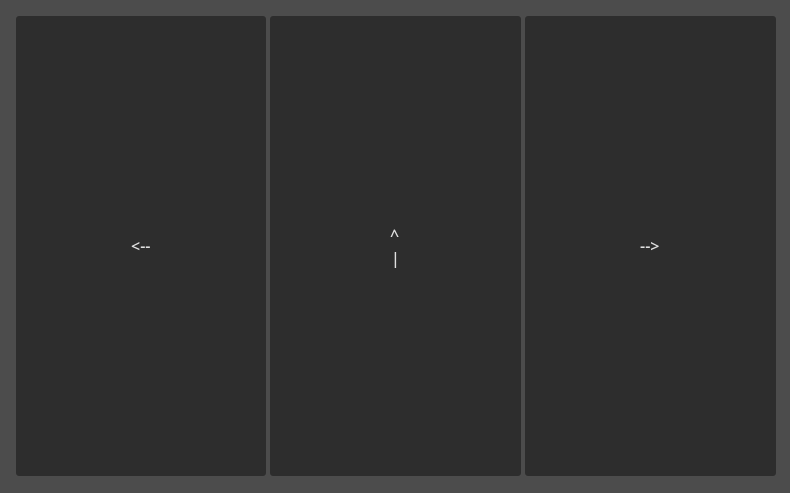
\includegraphics[width=\textwidth]{figuras/mapa_salas_sin.png}
		\caption{Puzle de salas en su versión de un jugador.}
		\label{fig:mapa_salas_sin}
	\end{minipage}
\end{figure}
En la versión para dos jugadores, representada en la figura \ref{fig:mapa_salas_mul}, está disponible un entorno con las tres direcciones y sus baldosas correspondientes, pero el jugador que controla al personaje es incapaz de escuchar el sonido que las identifica, dependiendo del otro jugador para definir la dirección a la que moverse. \\

En la versión para un solo jugador, disponible en la figura \ref{fig:mapa_salas_sin},  se presentan tres botones que indican las tres direcciones disponibles para el jugador. Enfocar un botón describiría la estética de las baldosas, mientras que el cambio de sala se indica con una transformación del sonido ambiental. Si se selecciona la baldosa incorrecta, se vuelve al inicio. \\

\subsubsection{Sexta y última iteración}
En esta última iteración, se revisaron todos los puzles y se creó el fin del juego. Para finalizarlo, es necesario resolver todos los puzles y obtener dos objetos clave que se insertan en una puerta en la parte inferior del mapa. De esta manera, los jugadores deben resolver los distintos retos en el orden que deseen para completar el juego y prueban así las estrategias sonificadas en su totalidad. \\

Al crear los binarios, se distribuyeron a los usuarios finales para realizar las pruebas y la encuesta de accesibilidad. Se descubrió que la configuración de los lectores de pantalla en el ordenador de los usuarios ciegos hacía que el juego no reprodujera las líneas de texto necesarias para los tutoriales y los puzles, haciéndolo injugable. Para mitigar esto, se cambió el uso de un TTS por líneas pregrabadas de audio para todos los textos. \\
\section{Pruebas finales de usuario}
%TODO redactar pruebas
Para comprobar la eficacia de las estrategias de sonificación implementadas, se buscó la colaboración con distintas organizaciones relacionadas con la ayuda a personas con visión reducida o nula. Después de acordar dicha colaboración, se realizó una solicitud al comité de ética de la Universidad de Granada describiendo la naturaleza de estas pruebas, los datos que se iban a recolectar y la muestra de usuarios esperada. Se contactó con la ONCE, que a su vez redirigió la información al proyecto de Modos-ON.\\

El grupo de Modos-ON \cite{BienvenidosModosONActivando} es una iniciativa del centro de tiflotecnología e innovación de la ONCE dedicado al análisis de la accesibilidad y jugabilidad de personas con ceguera en videojuegos. Su experiencia creando informes sobre videojuegos profesionales supuso una gran ayuda para esta sección del trabajo. \\

Debido a que este grupo está ubicado en Madrid, se diseñaron pruebas de usuario remotas y se realizaron reuniones de seguimiento virtuales a través de las cuales se compartían dudas y sugerencias sobre el juego. Puesto que no fue posible estar presente durante la realización de las pruebas, se diseñó una encuesta de accesibilidad disponible en el Anexo A que los usuarios pudieran cumplimentar al terminar el juego. \\

Los resultados de esta encuesta están disponibles en el siguiente enlace \footnote{\url{https://docs.google.com/spreadsheets/d/1VDdT31XRfZXDO9eVwdrws6TXJwX1hXIXhNrKS8BGuA0/edit?usp=sharing}}, dispuestos en una tabla de datos en la que cada columna corresponde a una pregunta y cada fila a usuarios que han respondido a la encuesta. \\

Puesto que la limitación temporal del trabajo exige su publicación en fechas específicas, la aprobación del comité de ética se requería previa a las pruebas y se necesitó de una búsqueda exhaustiva y del contacto de múltiples organizaciones, las pruebas están realizándose en el momento de publicar este trabajo. Esto supone una menor muestra en la encuesta y no es posible analizarla estadísticamente. Sin embargo, se analizarán las respuestas y las mejoras potenciales del juego en base a la experiencia de los usuarios en la sección de conclusiones. \\

En el momento de publicación de este trabajo, se han realizado tres pruebas completas con tres personas con visión reducida y son sus respuestas a la encuesta las que se analizarán en las conclusiones. Las pruebas se realizaron en la versión de un solo jugador con teclado.\\
